\hypertarget{modelling-reactive-behavior-notation---state-inspection}{%
\section{Modelling Reactive Behavior Notation - State
Inspection}\label{modelling-reactive-behavior-notation---state-inspection}}

\textbf{State-inspection is one of three synchronous mechanisms for interaction between reactive-objects}

\begin{itemize}
\tightlist
\item
  Many transitions with the same Trigger (In-pulse or event-message)
\item
  Is not deterministic -\textgreater{} needs a condition to specify in
  which case which transition is taken
\item
  The condition for a transition, e.g. {[}canHeat{]}, is called Guard in
  UML
\item
  canHeat is a boolean function, in CIRO called Gate
\item
  In our example canHeat should be true if switch is in state On and
  tank is in state Full
\item
  To evaluate the gate, the state of other objects has to be inspected
\item
  For this reason in CIRO this interaction is called State-Inspection
\end{itemize}

\hypertarget{definition-of-state-inspection-interaction}{%
\subsection{Definition of
State-Inspection-Interaction}\label{definition-of-state-inspection-interaction}}

\begin{itemize}
\tightlist
\item
  The heatingControl does not know, when canHeat is true or false
\item
  The value of the gate is based on a logical expression based on the
  states of inspected objects
\item
  We can only have one inspecting object, but we can have one or more
  inspected objects
\end{itemize}

\begin{figure}[H]
\centering
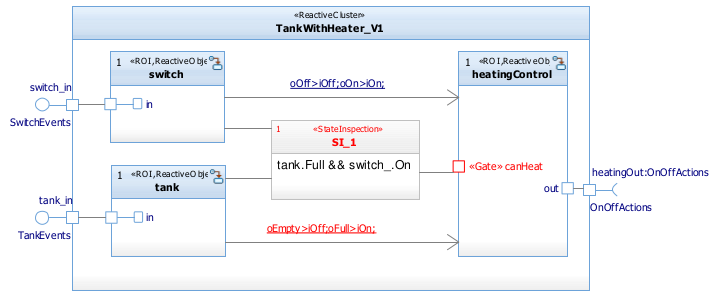
\includegraphics[width=1\textwidth]{figures/gateStateInspection.png}
\caption{State Inspection}
\end{figure}

\clearpage
\hypertarget{summary}{%
\subsection{Summary}\label{summary}}

\begin{itemize}
\tightlist
\item
  Transition branch depends on states of other objects
\item
  Synchronous interaction
\item
  Only within cluster
\item
  One inspecting object
\item
  Many inspected objects
\item
  Gate defines interface of boolean function, the logical expression is
  defined within as part of the state inspection connection
\item
  Gate belongs to the interface of the inspecting object
\item
  Gate is used to define guards, i.e.~conditions for transition branches
\end{itemize}

\clearpage